\section{Resultat}
I den här delen av rapporten kommer resultaten att presenteras. Resultatet redovisas kategorivis utefter Laugwitz et al. \cite{Laugwitz2008ConstructionQuestionnaire} bedömning av användarupplevelse, en riktlinje som använts i denna rapport, vilket är: 
\begin{itemize}
\item Tydlighet
\item Attraktivitet
\item Stimuli
\item Effektivitet
\item Pålitlighet
\end{itemize}
Resultat från både enkätundersökningar och fokusgrupper kommer att redovisas.
För mer information om kategorierna se avsnitt \ref{kategorisering}.\\

Av de 60 personer som enkäten skickades ut till fick vi 24 svar.  15 människor kunde samlas till fokusgrupperna med fem deltagare i vardera grupp under tre tillfällen. \\

% Sammanställningen av resultatet är i tre delar, där första delen är ett stapeldiagram på hur värdeskapande/viktigt kategorin är för slutanvändarens användarupplevelsen. Hur viktigt en specifik i varje kategori är blir representerat på en skala från 1-10 där en 10a är högsta betyg. Ju högre betyg det är för en kategori desto viktigare är den delen för användarupplevelsen. 
% \\

% Den andra delen är en bild som visar utvärderingen på AL1. Först visas medelvärdet som besvarar frågan, \textit{hur viktigt användarupplevelsen är}. Det följs av utvärderingen på prototypen som är en sammanställning på enkätfrågorna. Figuren representerar en total på de olika svarsalternativen 1-6 där en 6a är högsta betyg. Ju högre betyg det är för en kategori desto positivare har användarupplevelsen varit. 
% \\

% Sist kommer resultatet från fokusgrupperna. Vad fokusgrupperna diskuterade presenteras nedan grupperat efter kategori. Med utvalda citat för varje del.\\

% För hela diskussionerna av fokusgrupperna och enkätundersökningens frågor se bilaga A och B.
 
\subsection{Tydlighet}
Hur viktigt tydlighet är för användarupplevelsen är representerat från 1-10 där 10 är högsta betyg. Ju högre betyg det är för en kategorin desto viktigare är det för användarupplevelsen. Stapeldiagrammet presenteras i procentsatser för att ge en bättre översikt. 
\newline

\centerline{\textbf{Hur viktigt är tydlighet för 
din användarupplevelse}}
\begin{figure} [H] 
  \centering
  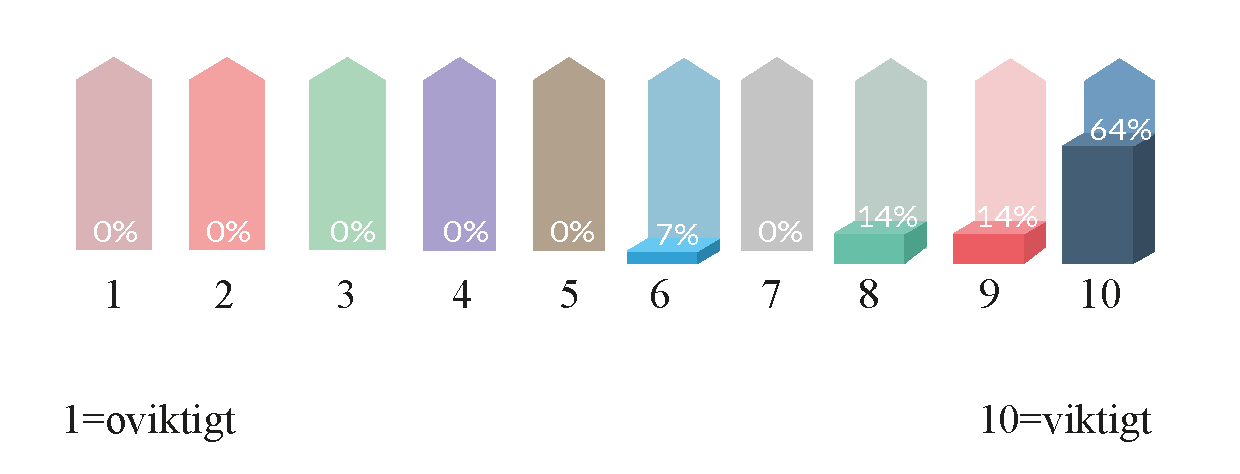
\includegraphics[scale=0.7]{Rityta_10.pdf}
\centering
\captionsetup{justification=centering,margin=2cm}
\caption{Resultat i procentuell skala på respondenternas svar}
\end{figure} 

Medelvärdet av ovan figur är 9.29. Siffran representerar ett medelsnitt av stapeldiagrammet som visar hur viktigt det var för användarupplevelsen enligt kategoriseringen framtagen av Hazzendahl. 


\begin{figure} [H]
  \centering
  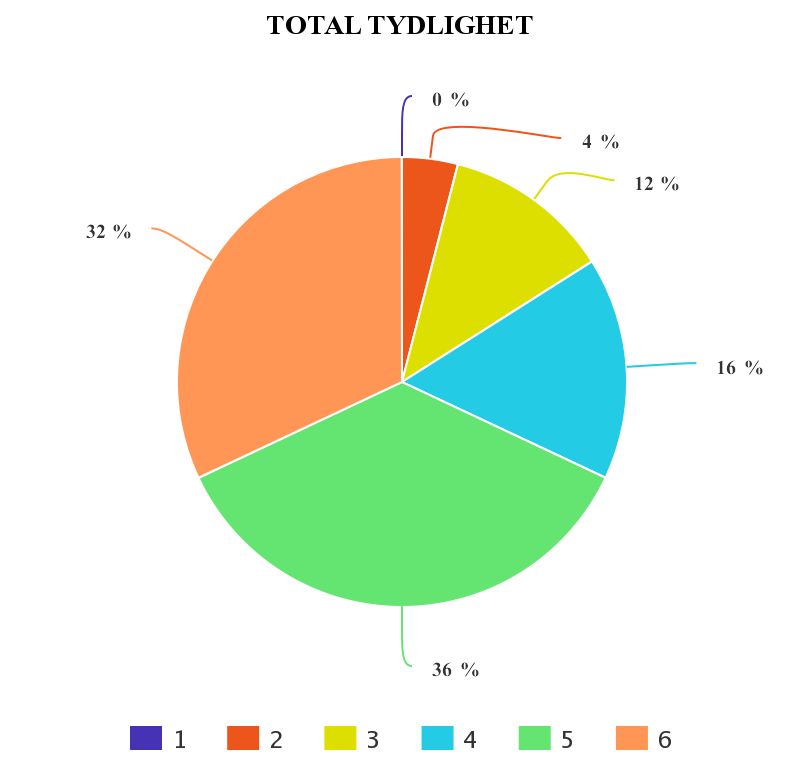
\includegraphics[scale=0.4]{meta-chart-2.png}
 \captionsetup{justification=centering,margin=2cm}
 \caption{Resultat av total tydlighet}
\end{figure} 



\begin{figure} [H]
  \centering
  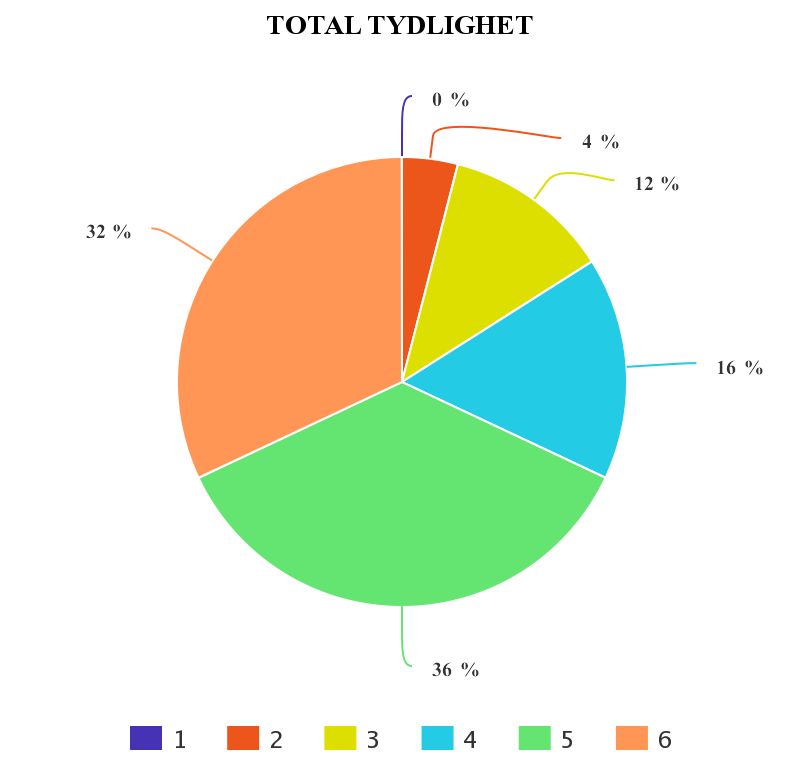
\includegraphics[scale=0.4]{meta-chart-2.png}
 \captionsetup{justification=centering,margin=2cm}
 \caption{Resultat av total tydlighet}
\end{figure} 

Figuren visar det slutgiltiga resultatet från både enkätundersökningen samt fokusgrupperna. Figuren visar sambandet mellan hur viktigt tydlighet är för användarupplevelsen i en applikation kontra hur tydlig prototypen känts. Den första rutan visar på hur viktigt det är för användaren att en applikation är tydlig, enligt personerna som medverkade i fokusgrupperna. Denna siffran beräknades med hjälp av snitt och varians och presenteras nedan. Diagrammen visar på hur tydlig prototypen kändes, enligt användarna som svarade på enkätundersökningen. 
\newline

\textbf{Citat från fokusgrupperna}
\begin{quotation}
\em Det var inte glasklart vart man ska markera, för det fanns ingen punkt eller checkbox
\end{quotation}

\begin{quotation}
\em Sen kan man ju tänka sig att ser man dåligt så är det lite för grått, texten är för grå.
\end{quotation}

\begin{quotation}
\em Man förstod att det var en film man skulle kolla på i och med att det var en playknapp. Inte svårt att förstå men jag fick inte sammanhanget. The why, varför gör jag detta, om jag får reda på det så kör jag vidare sedan utan att tänka.
\end{quotation}


%\begin{quotation}
%\em % hur många gånger ska jag göra de här övningarna? 
%\end{quotation}

%\begin{quotation}
%\em %Jag vill alltid tänka att ”vad är minimal effort för att gå vidare från detta”? 
%\end{quotation}

%\begin{quotation}
%\em %ja det är bra att se hur lång resan är. 
%\end{quotation}

%\begin{quotation}
%\em %Men det fanns ingen övergripande på dessa tre minuterna, det saknades ju helt. Det var på enskilda moment fanns det ju så att man kunde gissa sig fram på hur lång det var men inte helheten. 
%\end{quotation}

%\begin{quotation}
%\em %I think that it was not that clear, you have to be more clear in the beginning of what the goals for this exercise is. What is the goal and mission.  Why are you starting here? What is the steps? And I think it’s important to visualize it. 
%\end{quotation}
